\documentclass[tikz,border=0pt]{standalone}
\usepackage{tikz}

% --- COLOR DEFINITIONS ---
\definecolor{Garnet}{HTML}{73000A}
\definecolor{CBlue}{HTML}{466A9F}
\definecolor{CGrayDark}{HTML}{555555}

\begin{document}
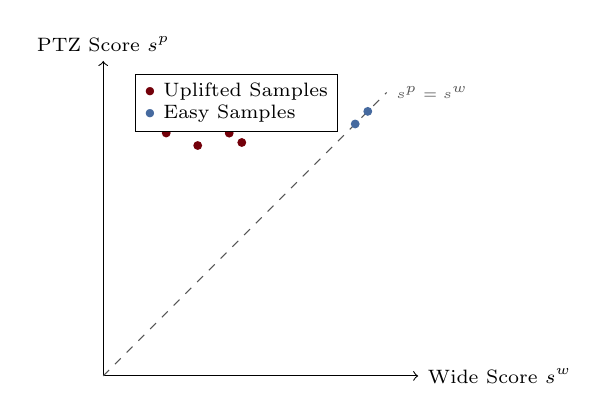
\begin{tikzpicture}[scale=0.8]
  \draw[->] (0,0) -- (5,0) node[right, font=\scriptsize] {Wide Score $s^w$};
  \draw[->] (0,0) -- (0,5) node[above, font=\scriptsize] {PTZ Score $s^p$};
  \draw[dashed, CGrayDark] (0,0) -- (4.5,4.5) node[right, font=\tiny] {$s^p = s^w$};

  % Low conf wide, High conf PTZ
  \foreach \x in {1, 1.2, 1.5, 2.0, 2.2} {
     \fill[Garnet] (\x, {3.5 + rand*0.5}) circle (2pt);
  }
  % Med conf wide, High conf PTZ
  \foreach \x in {2.5, 3.0, 3.2} {
     \fill[Garnet] (\x, {4.0 + rand*0.3}) circle (2pt);
  }
  % High conf both
  \foreach \x in {4.0, 4.2} {
     \fill[CBlue] (\x, \x) circle (2pt);
  }

  \node[align=left, font=\scriptsize, fill=white, draw=black, anchor=north west] at (0.5, 4.8) {
     \textcolor{Garnet}{$\bullet$} Uplifted Samples\\
     \textcolor{CBlue}{$\bullet$} Easy Samples
  };
\end{tikzpicture}
\end{document}
